%implementing document formatting:
%page setup (page size, text size, page layout, chapters start on a new page).
%memoir is a form of book class that supports any kind of document.
\documentclass[fleqn,a4paper,12pt,twoside,openany]{memoir}
\usepackage[footnote,draft,danish,silent,nomargin]{fixme}
\usepackage{titlesec}
\usepackage{anysize}
\usepackage{enumitem}

\usepackage{pifont} % extra symbols like (v.. approved)...
\usepackage[hyphens]{url}
\usepackage{array}
\usepackage{multirow}

%\titleformat{\chapter}[display]
%{\normalfont\huge\bfseries}{\chaptertitlename\ \thechapter}{20pt}{\Huge}

% this alters "before" spacing (the second length argument) to 0

\titlespacing*{\chapter}{0pt}{-50pt}{10pt}


%setting the header and footer in that order:
\setheadfoot{28pt}{28pt} %if any problems are encountered, try changing the latter 28pt with 1cm.

%general package syntax: \usepackage[options]{package}

%setting language:
\RequirePackage[danish, english]{babel}

%this package makes it possible to treat any element as a float,
%figures and tables are by default treated as floats.
%read http://en.wikibooks.org/wiki/LaTeX/Floats,_Figures_and_Captions to specify your float.
\usepackage{float}
\usepackage{wrapfig}
\usepackage{placeins}
\usepackage{siunitx}


%this package makes it possible to make theorems and examples:
\usepackage{amsthm}
%setting the style of examples (parameters: plain, definition, remark):
%(definition is usually used for examples)
\theoremstyle{definition}
%the frist parameter is the syntax used in the document, the second is that which is printed in LaTex.
\newtheorem{example}{Example}

%making it possible to use æ, ø and å:
\usepackage[utf8]{inputenc}
%helps with word division when using æ, ø and å, and makes it ps-font rather than bmp:
\usepackage[T1]{fontenc}

%package for implementation of graphic files:
\usepackage{graphicx}

%package for captions
\usepackage[nooneline]{caption}
\captionsetup[table]{name=Tabel}
\captionsetup[figure]{name=Figur}
\usepackage{subcaption}

%%package for implementation of math:
\usepackage{amsmath, amsfonts, amssymb, float, mathtools}

%allowing use of color:
\usepackage[usenames,dvipsnames]{color}
%allowing use of more colors also in tables (see: http://en.wikibooks.org/wiki/LaTeX/Colors):
\usepackage[usenames,dvipsnames,svgnames,table]{xcolor}
\usepackage{colortbl} %Colors for tabulars
\definecolor{pwdrblue}{RGB}{140,140,140} %Color changed back!
\definecolor{darkgrey}{RGB}{180,180,180}
\definecolor{lightgrey}{RGB}{201,201,201}
\definecolor{aaublue}{RGB}{53,46,102}
\definecolor{aausub}{RGB}{154,167,180}
\definecolor{MidnightBlue}{RGB}{25, 25, 112}
\definecolor{NavyBlue}{RGB}{0, 0, 128}
\definecolor{darkgray}{gray}{0.35}
\definecolor{AleeRed}{rgb}{0.5,0,0}
%hyperlinks in the tabel of contents - comment this out before the report is printed.
\usepackage{hyperref}
\hypersetup{
	bookmarks = true,  % Show 'bookmark'-frame in pdf.
	colorlinks = false, % True = colored links, False = framed links.
	citecolor = blue,  % Link color for references.
	linkcolor = blue,  % Link color in table of contents.
	urlcolor = blue,   % Link color for extern URLs.
}

%makes it possible to refer to the name of a chapter rather than just the number.
\usepackage{nameref}
\usepackage[american,cuteinductors,smartlabels]{circuitikz}
\usepackage{tikz}
\usetikzlibrary{shapes,arrows,positioning,calc}
\usetikzlibrary{calc}
\usetikzlibrary{patterns}

%package for writing program code in latex
\usepackage{listings}

\lstset{ 
language=C,               	 	% choose the language of the code
basicstyle=\footnotesize,       % the size of the fonts that are used for the code
numbers=left,                   % where to put the line-numbers
numberstyle=\footnotesize,      % the size of the fonts that are used for the line-numbers
stepnumber=1,                   % the step between two line-numbers. If it is 1 each line will be numbered
numbersep=5pt,                  % how far the line-numbers are from the code
backgroundcolor=\color{white},  % choose the background color. You must add \usepackage{color}
showspaces=false,               % show spaces adding particular underscores
showstringspaces=false,         % underline spaces within strings
showtabs=false,                 % show tabs within strings adding particular underscores
frame=single,           		% adds a frame around the code
tabsize=2,          			% sets default tabsize to 2 spaces
captionpos=b,           		% sets the caption-position to bottom
breaklines=true,       			% sets automatic line breaking
breakatwhitespace=false,    	% sets if automatic breaks should only happen at whitespace
escapeinside={\%*}{*)}          % if you want to add a comment within your code
}

\definecolor{dkgreen}{rgb}{0,.6,0}
\definecolor{dkblue}{rgb}{0,0,.6}
\definecolor{dkyellow}{cmyk}{0,0,.8,.3}

\lstset{
  language        = php,
  basicstyle      = \small\ttfamily,
  keywordstyle    = \color{dkblue},
  stringstyle     = \color{red},
  identifierstyle = \color{dkgreen},
  commentstyle    = \color{gray},
  emph            =[1]{php},
  emphstyle       =[1]\color{black},
  emph            =[2]{if,and,or,else},
  emphstyle       =[2]\color{dkyellow}}
%setting references (using numbers) and supporting i.a. Chicargo-style:

\usepackage{url}

\usepackage[backend=bibtex]{biblatex}
\bibliography{bibliography/bibliography.bib}

\usepackage{verbatim} %enables /begin(comment) and /end{comment} for larger sections

%this package makes it possible include pdf pages in fx appendix;
%using  following syntax: \includepdf[pages={1}]{myfile.pdf}
\usepackage{pdfpages}

\usepackage{pbox} % used for newline in tabular

%%%MARGINER%%%
\setlrmarginsandblock{3.5cm}{2.5cm}{*}	% \setlrmarginsandblock{inner margin}{outer margin}{ratio}
\setulmarginsandblock{2.5cm}{3.0cm}{*}	% \setulmarginsandblock{top}{bottom}{ratio}
\checkandfixthelayout 			            % fixes stuff..

%Enables the use FiXme refferences. Syntax: \fixme{...}
%With "final" in stead of "draft" an error will ocure for every FiXme
%under compilation.
%\usepackage[footnote,draft,english,silent,nomargin]{fixme}

%Centering captions in tables
%\centering
%\captionsetup{justification=centering}
%\caption{bla bla bla}
\usepackage{caption}
\usepackage{pgfplotstable}
\usepackage{pgfplots}

\pgfplotsset{width=15cm,height=7cm}
\usepackage{filecontents}
\usepackage{epstopdf}
\usepackage{nomencl}
\renewcommand{\nomname}{Ordliste}
\renewcommand*{\pagedeclaration}[1]{\unskip\dotfill\hyperpage{#1}}
\makenomenclature
\usepackage{makeidx}
\makeindex

%implementing macros:
%%Figure references:
\newcommand{\figref}[1]{\textbf{figur \ref{#1}}}

%Figure references after full stop/period:
\newcommand{\Figref}[1]{\textbf{Figur \ref{#1}}}

%Table references:
\newcommand{\tableref}[1]{\textbf{tabel \ref{#1}}}

%%%CHAPTERLAYOUT%%%
%setting the color of the chapter number
\definecolor{numbercolor}{gray}{0.7}
%Downloaded chapter-setup:
\newif\ifchapternonum
\makechapterstyle{jenor}{
	\setlength{\beforechapskip}{-2cm}	% Adjust space between page top and chapter title.
	\setlength{\afterchapskip}{1.5cm}	% Adjust spave between chapter title and text.
  	\renewcommand\printchaptername{}
  	\renewcommand\printchapternum{}
  	\renewcommand\printchapternonum{\chapternonumtrue}
  	\renewcommand\chaptitlefont{\fontfamily{pbk}\fontseries{db}\fontshape{n}\fontsize{25}{35}\selectfont\raggedleft}
  	\renewcommand\chapnumfont{\fontfamily{pbk}\fontseries{m}\fontshape{n}\fontsize{1in}{0in}\selectfont\color{numbercolor}}
  	\renewcommand\printchaptertitle[1]{%
    \noindent
    \ifchapternonum
    \begin{tabularx}{\textwidth}{X}
    {\let\\\newline\chaptitlefont ##1\par} 
    \end{tabularx}
    \par\vskip-2.5mm\hrule
    \else
    \begin{tabularx}{\textwidth}{Xl}
    {\parbox[b]{\linewidth}{\chaptitlefont ##1}} & \raisebox{-15pt}{\chapnumfont \thechapter}
    \end{tabularx}
    \par\vskip2mm\hrule
    \fi
  }
}
%setting chapter style:
\chapterstyle{jenor}

%depth of numbered headlines (part/chapter/section/subsection):
%\setsecnumdepth{subsection}
%\maxsecnumdepth{subsection}
%depth of the table of contents:
\settocdepth{section}
\parindent=0pt 

% Makes sure LaTeX does not stretch the text at page break:
\raggedbottom

\newcommand{\img}[4]{
    \begin{figure}[!ht]
    	\centering
    		\includegraphics[width=#4\textwidth]{#1}
    	\caption{\text{#2}}
    	\label{#3}
    \end{figure}
}

\newcommand{\tableimg}[3]{
    \begin{figure}[!ht]
    	\centering
    		\includegraphics[width=#3\textwidth]{#1}
    	\label{#2}
    \end{figure}
}

\newcommand{\wrapimg}[8]{
	\begin{wrapfigure}[10]{#5}{0.4\textwidth} \hspace{0pt}
	\vspace{#6}
  		\begin{center}
   			 \includegraphics[width=#4\textwidth]{#1}
  		\end{center}
  		\vspace{#7}
 		\caption{\textbf{#2}}
 	 	\label{#3}
 	 	\vspace{#8}
	\end{wrapfigure}
}

\newcommand{\sidebyimg}[4]{
	\begin{figure}[H]
		\center
		\begin{subfigure}[b]{0.48\textwidth}
			\includegraphics[width=\textwidth]{#1}
			\caption{#2}
		\end{subfigure}
		\quad
		\begin{subfigure}[b]{0.48\textwidth}
			\includegraphics[width=\textwidth]{#3}
			\caption{#4}
		\end{subfigure}
	\end{figure}
}

\newcommand{\sidebyimglabel}[8]{
	\begin{figure}[H]
		\center
		\begin{subfigure}[b]{0.48\textwidth}
			\includegraphics[width=\textwidth]{#1}
			\caption{#2}
			\label{#3}
		\end{subfigure}
		\quad
		\begin{subfigure}[b]{0.48\textwidth}
			\includegraphics[width=\textwidth]{#4}
			\caption{#5}
			\label{#6}
		\end{subfigure}
		\caption{#7}
		\label{#8}
	\end{figure}
}

\newcommand{\threesidebyimg}[9]{
	\begin{figure}[!htb]
		\minipage{0.32\textwidth}
  			\includegraphics[width=\linewidth]{#1}
  			\caption{\textbf{#2}}\label{fig:#3}
		\endminipage\hfill
		\minipage{0.32\textwidth}
  			\includegraphics[width=\linewidth]{#4}
  			\caption{\textbf{#5}}\label{fig:#6}
		\endminipage\hfill
		\minipage{0.32\textwidth}
  			\includegraphics[width=\linewidth]{#7}
  			\caption{\textbf{#8}}\label{fig:#9}
		\endminipage\hfill
	\threesidebyimgcontinued
}

\newcommand{\threesidebyimgcontinued}[1]{
	\caption{\textbf{#1}}
	\end{figure}
}

\newcommand{\blueheader}[1]{
	\cellcolor{aaublue}\textbf{\color{white}#1}
}
\begin{document}
\nomenclature{THT}{Through-hole technology}
\nomenclature{UART}{Universal asynhcronous reciever/transmitter}
\nomenclature{PCB}{Printet circuit board}
\nomenclature{PPM}{Parasite power mode}
\nomenclature{LSB}{Least significant bit}
\nomenclature{SQL}{Structured query language}
\nomenclature{HTML}{Hyper text markup language}
\nomenclature{UDP}{User datagram protocol}
\nomenclature{TCP}{Transmission control protocol}
\nomenclature{SPI}{Serial periphial interface}
\nomenclature{P2P}{Point to point}
\nomenclature{SMD}{Surface-mount device}

\renewcommand\chaptername{Kapitel}
\renewcommand\contentsname{Indholdsfortegnelse}
\renewcommand\figurename{Figur}
\renewcommand\tablename{Tabel} 

%implementing front page:
\clearpage
\thispagestyle{empty}

\begin{figure}[H]
	\raggedleft
		
\includegraphics[width=0.2\textwidth]{figures/logo-ucn.png}
\end{figure}
\vspace*{\fill} 
\begin{center}
\begin{Huge}
Forårs Semester 2016\\
\vspace{5 mm}
\textbf{Line following automotive robot}\\
\vspace{3 mm}
Gruppe 4\\
\vspace{3 mm}
2. Semester IT-Teknolog
\end{Huge}
\end{center}

\begin{figure}[h!]
  \centering
  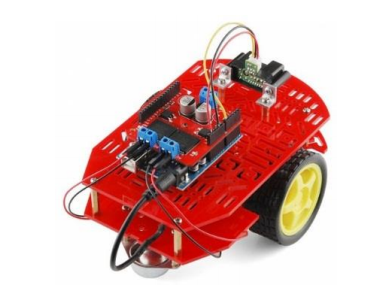
\includegraphics[width=0.7\textwidth]{figures/Produktet.png}
\end{figure}

\vspace*{\fill}
\begin{center}
Gruppe medlemmer:
 Anders Pedersen - Kasper Delfs - Kristian Porsborg
\end{center}
\begin{center}
Vejledere: Jesper M. Kristensen og Steffen Vutborg
\end{center}
\begin{center}
\line(1,0){400}
\end{center}
%clears one or two pages to make the document start on right hand side:
\cleardoublepage

%numbers the pages with Roman numeral - starts from "i":
\frontmatter

%implementing title sheet:
% Dette er LaTeX-versionen af titelbladet for tek-nat-basis-rapporter 2004 efterår
% Filen kræver:
% Universitetets logo:  aau-logo.png (for LaTeX) eller aau-logo.ps (for LaTeX)
% Synopsis: En fil ved navn synopsis.tex

% Udarbejdet af: Hans Håttel (hans@cs.auc.dk) 21. maj 2003
% Rettet af Morten Christophersen (mortench@tnb.aau.dk) 30. nov 2004(ændret til nyt design 2004 efterår)

%\documentclass[11pt]{article}
%\ifx\pdfoutput\undefined 
%\usepackage[dvips]{graphicx}
%\else
%\usepackage[pdftex]{graphicx} 
%\usepackage{type1cm} \fi
%    \usepackage[ansinew]{inputenc}
%    \usepackage{a4}

%\begin{document} 
\thispagestyle{empty}
%\begin{titlepage}
\begin{nopagebreak}
{\samepage 

\begin{tabular}{r}
\parbox{\textwidth}{  \raisebox{11mm}{
\includegraphics[height=1.5cm]{figures/logo-ucn.png}}
\hfill \hspace{2cm} \parbox{8cm}{\begin{tabular}{l} %4.90
{\small \textbf{\textcolor{MidnightBlue}{1. Semester}}}\\
{\small \textbf{\textcolor{MidnightBlue}{IT-teknolog}}}\\ 
{\small \textcolor{NavyBlue}{Sofiendalsvej 60}} \\
{\small \textcolor{NavyBlue}{9200 Aalborg SV}} \\
{\small \textcolor{NavyBlue}{\emph{http://www.ucn.dk/}}}
\end{tabular}}}
\end{tabular}

\begin{tabular}{cc}
\parbox{7cm}{
\begin{description}

\item { Titel:} 

Temperaturændringer på\\ vandledning

\end{description}

\parbox{8cm}{

\begin{description}
\item { Projekt Periode:}\\
   1. Semester | Vinter semester 2016\\
  \hspace{4cm}
\item { Projectgruppe:}\\
  Gruppe 1 
  \hspace{4cm}
\item { Medvirkende:}\\
Anders Pedersen\\
Benjamin Nielsen\\
Henrik Jensen\\
Kasper Delfs\\
Kristian Porsborg\\
\hspace{2cm}
\item { Vejleder:}\\
Jesper M. Kristensen og \\Steffen Vutborg
  
\end{description}
}
\begin{description}
\item { Sideantal: TBD} \fxnote{indsæt sideantal}
\item { Appendiks: TBD} \fxnote{indsæt sideantal for appendiks}
\item { Færdiggjort: 21/1-2016}
\end{description}
\vfill } &
\parbox{7cm}{
  \vspace{.15cm}
  \hfill 
  \begin{tabular}{l}
   \end{tabular}}
\end{tabular}} \vspace{1.3cm}
\centering
\\
\end{nopagebreak}
%\end{titlepage}
%\end{document}
\chapter*{Forord}

%Læsevejledning:\\
%Kommer senere i projektforløbet.
%\\\\
Dette projekt er udarbejdet af en gruppe 1. semesterstuderende på uddannelsen
IT teknolog på UCN i efteråret 2015. Temaet i projektet er elektroniske systemer.





%
\phantom{Luft}\vspace{3cm}
\begin{table}[H]
	\centering
		\begin{tabular}{c c c}
			\underline{\phantom{JAERJAERJAERJAERGO}} & \phantom{cookies} & \underline{\phantom{JAERJAERJAERJAERGO}} \\
			Anders Pedersen			& \phantom{cookies} & Benjamin Nielsen		\\
			&&\\
			&&\\
			\underline{\phantom{JAERJAERJAERJAERGO}} & \phantom{cookies} & \underline{\phantom{JAERJAERJAERJAERGO}} \\
			Henrik Jensen			& \phantom{cookies} & Kasper Delfs		\\
			&&\\
			&&\\
	    \underline{\phantom{JAERJAERJAERJAERGO}} & \phantom{cookies} & \\
			Kristian Porsborg  					 
			&&\\							
		\end{tabular}
\end{table}

\cleardoublepage

%the '*' allows the tableofcontents be excepted from the actual table of contents.
\tableofcontents*
\newpage
\printnomenclature
\renewcommand*\listfigurename{Figurliste}
\renewcommand*\listtablename{Tabelliste}

%numbers the pages with Arabic numeral - starts from 1.
\mainmatter
\chapter{Foranalyse}
\section{Indledning}
Skriv noget her om hvorledes projektet kan afhjælpe automatisering i samfundet
\section{Line Track}


\chapter{Kravspecifikation}
I det følgende afsnit gives der indblik i de krav som er sat i problemanalysen samt de krav projektgruppen har sat for at imødegå produktet præsenteret i projektbeskrivelsen.

\subsection{Generelle krav}  
\begin{enumerate}
\item Projektet skal konstrueres omkring Sparkfun's Magician Chassis hvor to dc motorer er inkluderet.
\item Til projektet skal en mikrocontroller anvedes baseret på mikroprocessoren PIC32MX 32bit.
\item Produktet skal fremvises og demonstreres til projektevalueringen.
\item Projektet skal dokumenteres i form af en rapport.
\end{enumerate}

\subsection{Krav til produktet}
\begin{enumerate}
\item Produktet skal være i stand til køre på en linje med en minimumsbredde på 30 mm. 
\begin{enumerate}
\item Styring skal foregå ved hjælp af feedback fra en eller flere lyssensorer.
\item Farven på linjen skal være sort eller gråtonet over 75\%.  Den omkring liggende farve skal være hvid eller gråtonet under 50\%.
\end{enumerate}
\item Softwaren til produktet skal skrives i MPLAP.
\end{enumerate}


\chapter{Hardware}
\section{Software Overblik}
Den indlende idé til en softwareløsning som kan følge en linje er udarbejdet, og ses på figur \ref{init_software}.

\begin{figure}[h!]
  \centering
  \includegraphics[width=0.6\textwidth]{figures/intisliserendeLoesning.png}
  \caption{Den inledende software løsning til linetrackinging med 1 sensor.}
  \label{init_software}
\end{figure}



\section{Sensor}
\section{Motor}
\section{PID regulering}
For at opnå en mindskning i fejl målingerne fra sensoren,  kan indplementeres en PID. PID står for Proportional Integral Derivative controller. Formålet med en PID er at man konstant måler en fejl værdi som består af differensen mellem en ønsket værdi og en målt værdi. PID'en forsøger at minimere fejlmålingerne ved at justerer fejl målingen over tid.\newline
\newline
PID kan opskrives på følgende måde.

\begin{equation} 
u(t) = K_p e(t) + K_i\int_{0}^{t}e(T)dT + K_d\frac{\mathrm{d} e(t)}{\mathrm{d} t}
\end{equation}\label{PID}
\newline
hvor,
\newline
$K_{p}$, er proportional leddet som beskriver den nuværende værdi, hvilket er den ønskede værdi trukket fra den målte værdi. 
\newline
$K_{i}$, er integralleddet som beskriver den forhændværende værdi, hvilket betyder at fejlværdien bliver justreret ind over tid, dette gøres ved hjælp af det ønskede signal i forhold til det givet signal, som drager et areal af hver periode.   
\newline
$K_{d}$, er differentiale leddet som beskriver en mulig fremtidig fejl, som er vuderet ud fra forhændværende værdier. Dette gøres ved at måle hældningen på det givne signal for at forsøge at justere det ind efter den ønskede værdi. 
\newline

   
\section{Test}





\chapter{Software}
\section{Software Overblik}
Den indlende idé til en softwareløsning som kan følge en linje er udarbejdet, og ses på figur \ref{init_software}.

\begin{figure}[h!]
  \centering
  \includegraphics[width=0.6\textwidth]{figures/intisliserendeLoesning.png}
  \caption{Den inledende software løsning til linetrackinging med 1 sensor.}
  \label{init_software}
\end{figure}



\section{Sensor}
\section{Motor}
\section{PID regulering}
For at opnå en mindskning i fejl målingerne fra sensoren,  kan indplementeres en PID. PID står for Proportional Integral Derivative controller. Formålet med en PID er at man konstant måler en fejl værdi som består af differensen mellem en ønsket værdi og en målt værdi. PID'en forsøger at minimere fejlmålingerne ved at justerer fejl målingen over tid.\newline
\newline
PID kan opskrives på følgende måde.

\begin{equation} 
u(t) = K_p e(t) + K_i\int_{0}^{t}e(T)dT + K_d\frac{\mathrm{d} e(t)}{\mathrm{d} t}
\end{equation}\label{PID}
\newline
hvor,
\newline
$K_{p}$, er proportional leddet som beskriver den nuværende værdi, hvilket er den ønskede værdi trukket fra den målte værdi. 
\newline
$K_{i}$, er integralleddet som beskriver den forhændværende værdi, hvilket betyder at fejlværdien bliver justreret ind over tid, dette gøres ved hjælp af det ønskede signal i forhold til det givet signal, som drager et areal af hver periode.   
\newline
$K_{d}$, er differentiale leddet som beskriver en mulig fremtidig fejl, som er vuderet ud fra forhændværende værdier. Dette gøres ved at måle hældningen på det givne signal for at forsøge at justere det ind efter den ønskede værdi. 
\newline

   
\section{Test}





\chapter{Embedded}
\section{Software Overblik}
Den indlende idé til en softwareløsning som kan følge en linje er udarbejdet, og ses på figur \ref{init_software}.

\begin{figure}[h!]
  \centering
  \includegraphics[width=0.6\textwidth]{figures/intisliserendeLoesning.png}
  \caption{Den inledende software løsning til linetrackinging med 1 sensor.}
  \label{init_software}
\end{figure}



\section{Sensor}
\section{Motor}
\section{PID regulering}
For at opnå en mindskning i fejl målingerne fra sensoren,  kan indplementeres en PID. PID står for Proportional Integral Derivative controller. Formålet med en PID er at man konstant måler en fejl værdi som består af differensen mellem en ønsket værdi og en målt værdi. PID'en forsøger at minimere fejlmålingerne ved at justerer fejl målingen over tid.\newline
\newline
PID kan opskrives på følgende måde.

\begin{equation} 
u(t) = K_p e(t) + K_i\int_{0}^{t}e(T)dT + K_d\frac{\mathrm{d} e(t)}{\mathrm{d} t}
\end{equation}\label{PID}
\newline
hvor,
\newline
$K_{p}$, er proportional leddet som beskriver den nuværende værdi, hvilket er den ønskede værdi trukket fra den målte værdi. 
\newline
$K_{i}$, er integralleddet som beskriver den forhændværende værdi, hvilket betyder at fejlværdien bliver justreret ind over tid, dette gøres ved hjælp af det ønskede signal i forhold til det givet signal, som drager et areal af hver periode.   
\newline
$K_{d}$, er differentiale leddet som beskriver en mulig fremtidig fejl, som er vuderet ud fra forhændværende værdier. Dette gøres ved at måle hældningen på det givne signal for at forsøge at justere det ind efter den ønskede værdi. 
\newline

   
\section{Test}





\chapter{Test}
% mplab virker ikke 
% -> ADC fungere perfekt 
% -> PWM nåede ikke helt, 
% -> sat sammen virkede slet ikke
% pga. step by step -> har det forrige der virker
Under videreudviklingen og overførslen til MPLAB's platform mødte gruppen hindring i implementeringen deraf. En samlet test var ikke mulig, da der var problemer med opsætning af PWM modulet. ADC modulet fungerede efter hensigten, med korrekte målinger på 3 pins. Opsætningen af PWM modulet  blev ikke færdig udviklet pga. manglende tid. Dette betød at en samlet test ikke var mulig at udføre.
\\
\\
Som afslutning på projektet blev et race track event afholdt, hvor robottens evne til at følge en linje testet. Til denne test valgte gruppen at benytte den funktionelle arudino kode, som allerede var testet. Dog var koden ikke blevet testet i 90 grader sving, så derfor blev koden tweaket så dette var muligt.

% intro
% arudino, ikke mplab
% lille ændring i kode
% simpel kode uden PID
% 





%Efter overførslen af produt <Den samlede test af koden i MPlab var ikke sucessfuld, PWM modulet reagerede ikke korrekt ud fra de målte ADC værdier. Opsætningen af PWM modulet  blev ikke færdig testet pga. det var svært at finde information om omkring plib. Der blev taget udgangspunkt i et eksempel fra plib hjælpe dokumentet, samt datablad omkring opsætning af output compare.

\chapter{Konklusion}
I dette projekt havde gruppen til formål at designe og implementere den nødvendige hard- og software med henblik på at konstruere en automatisk linjefølgende robot.
\\
\\
Produktet er udviklet ud fra Magician chassis som blev leveret af Sparkfun med en dertil forud bestemt lyssensor. Produktet blev udviklet over flere stadier hvoraf den indledene fase var at implementere en sensor til en Arduino og få robotten til at følge linjen ud fra den feedback som kom fra sensoren. 
\\
Herfra implementerede gruppen flere sensore til produktet i form af videreudvikling af projektet. Dette resulterede i...... blah blah blah....

\chapter{Perspektivering}
Ved udviklingen af den linjefølgende robot har projektgruppen valgt at fokusere på at udvikle produktet skridt for skridt. Ved at anvende denne fremgangsmåde har det betydet at meget tid er gået med udviklingen og dokumentation af de forskellige stadier. Arduino kunne have været benyttet til blot at verificere at hardwaren fungere, og flytte fokus til implementering af software i MPLAB.
\\
\\
Det kunne være interessant at anvende yderligere sensorer, samt at sænke  afstanden mellem de monteret sensorer for få højere præcision, når roboten krydser linjen.







%\newpage
%\listoffigures
%\addtocontents{lof}{~\hfill\textbf{Page}\par}
%\newpage
%\listoftables
%\addtocontents{lot}{~\hfill\textbf{Page}\par}
\newpage
\printbibliography
\chapter{Appendix}
123
\includepdf[pages=-]{contents/appendix/side47.pdf}
\includepdf[pages=-]{contents/appendix/side14_15steps.pdf}
\includepdf[pages=-]{contents/appendix/line_follow_arduino.pdf}
\includepdf[pages=-]{contents/appendix/line_follow_embedded.pdf}
\newpage
\listoffixmes
\end{document}